\subsection{\label{sec:data.calib.systems}Subsystem Calibrations}

The raw \abbr{TDC} time ($t_\mathtt{TDC}$) from any particular element in the detector is related to the event start time ($t_\mathrm{start}$) by the equation:
\begin{equation}
    t_\mathtt{TDC} = t_\mathrm{start} + t_\mathrm{flight} + t_\mathrm{prop} + t_\mathrm{walk} + t_\mathrm{elec},
    \label{eqn:detector_time}
\end{equation}
where $t_\mathrm{flight}$ is the flight time of the particle from the reaction vertex to the element such as a scintillator paddle or layer in the drift chamber, $t_\mathrm{prop}$ is the propagation time of the signal from the track to the detection electronics (\abbr{PMT}s or readouts at the ends of the wires in the \abbr{DC}), $t_\mathrm{walk}$ (called the \emph{time walk}) is the time it takes the discriminator to recognize the signal as a ``hit,'' and $t_\mathrm{elec}$ is the final electronics delay due to cable lengths and signal relays and is generally a constant for all particles at all momenta. The term of interest, $t_\mathrm{start}$, is by definition the same for all hits in an event, however, it contains an arbitrary offset because it is a function of the trigger and therefore varies from event to event. The three times: $t_\mathrm{flight}$, $t_\mathrm{prop}$ and $t_\mathrm{walk}$ are all functions of the momenta and masses of the particles passing through the detector elements. The approximate magnitudes of each term in Eq.~\ref{eqn:detector_time} is shown in Table~\ref{tab:timings}.

\begin{table}
\begin{minipage}{\textwidth}
\begin{center}
\begin{singlespacing}

\caption[Single Timing Relationships]{\label{tab:timings}Relative timing relationships for the terms of Eq.\ref{eqn:detector_time}. The time ranges are the approximate correction amplitudes applied to the data. The column ``fn.\ of \abbr{PID}'' indicates if the time is dependent on the particle mass or momentum.}

\begin{tabular}{lrcp{25ex}}

\hline \hline

term & approx.\ range & fn.\ of \abbr{PID}? & description \\

\hline

$t_\mathtt{TDC}$ & 0--400~ns & no & recorded time by the electronics \\
$t_\mathrm{start}$ & 0--400~ns & no & event start time \\
$t_\mathrm{flight}$ & 20--50~ns & yes & particle flight time from vertex \\
$t_\mathrm{prop}$ & 0.1--10~ns & yes & signal propagation time \emph{to} electronics \\
$t_\mathrm{walk}$ & 100--400~ps & yes & descriminator response time \\
$t_\mathrm{elec}$ & 0.1--10~ns & no & signal propagation time \emph{in} electronics \\

\hline \hline

\end{tabular}

\end{singlespacing}
\end{center}
\end{minipage}
\end{table}
\vspace{20pt} % tab:timings

The goal of the timing calibrations was to determine all the values in Eq.~\ref{eqn:detector_time} for each detector element as a function of particle momentum, charge and/or mass when neccessary. The actual value of interest is always the flight time of the particles from the reaction vertex to the detector element ($t_\mathrm{flight}$) but the trigger offset inherent in $t_\mathrm{start}$ requires the use of the sum: $t_\mathrm{flight} + t_\mathrm{start}$. Only differences in these times (i.e. between two hits in the detector) were used in this analysis so that the trigger offset could be subtracted.

The two times in Eq.~\ref{eqn:detector_time} that are the most difficult to determine were $t_\mathrm{prop}$ and $t_\mathrm{walk}$. The first of these, the propagation time of the signal from the track to the electronics interface, is a property of the medium such as the gas or scintillator material. For double-ended paddles like in the \abbr{TOF}, this term was eliminated by taking the average of the \abbr{TDC} times from the two sides. The start counter which has \abbr{PMT}s on only one side of the scintillator paddles uses the intersection of the track from the \abbr{DC} information to determine this correction. The \emph{time walk} term ($t_\mathrm{walk}$) is a small ($<5\%$) correction which represents the electronic's interface response time to a physical signal and is a function of the \abbr{ADC} pulse height as discussed below.

Energy calibrations are generally determined using a known event sample within the data. The tagger energy, for example, was calibrated using the exclusive reaction:
\begin{equation}
    \mathrm{\gammaup p \rightarrow p \piup^+ \piup^-}\label{rxn:excl_ppippim}
\end{equation}
where the exclusivity was determined via missing momentum and missing mass cuts using the energy of the tagger hit associated with the event. The photon energy was then adjusted by taking the total energy of the $\mathrm{p \piup^+ \piup^-}$ system using the equation:
\begin{equation}
    E_\mathrm{beam, corrected} = E_\p + E_{\mathrm{\piup^+}} + E_{\mathrm{\piup^-}} - m_\p,
    \label{eqn:ebeam_ppippim}
\end{equation}
where $E_\p$, $E_{\mathrm{\piup^+}}$ and $E_{\mathrm{\piup^-}}$ are the energies of the outgoing particles, and $m_\p$ is the proton (target) mass. The average of at least 10k events per \emph{logical} tagger energy paddle (see Sec.~\ref{sec:clas.tagr}) was used for this correction and the results as a function of the beam energy is shown in Fig.~\ref{fig:data.calib.tag_energy}. The inherent resolution of the tagger paddles for \g12 was approximately 5.6~MeV.

Results from the tagger energy calibration were used to calculate corrections to the momenta of the tracks, the energy corrections were subsequently recalculated. This iterative process was employed several times until the values obtained for both corrections converged. The energy difference between $E_\mathrm{beam, corrected}$ in Eq.~\ref{eqn:ebeam_ppippim} and the energy reported by the tagger is shown in Fig.~\ref{fig:data.calib.ediff_ppippim}.

\begin{figure}\begin{center}
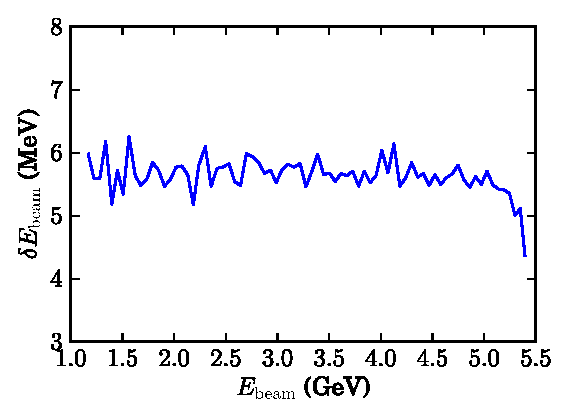
\includegraphics[width=0.55\columnwidth]{\figures/calibration/tagger/tagger_energies.eps}
\caption[\abbr{TAG} Energy Resolution vs.\ Beam Energy]{\label{fig:data.calib.tag_energy}Resolution of the \emph{logical} energy paddles in the tagger. The values were obtained by taking the difference in reported energy between two adjacent paddles. The unevenness can be attributed to overlapping regions of energy counters varying in size and the sagging of the $E$-counter plane\cite{clas.thesis.williams}. An average resolution of 5.6~MeV is indicated by this plot.}
\end{center}\end{figure}

\begin{figure}\begin{center}
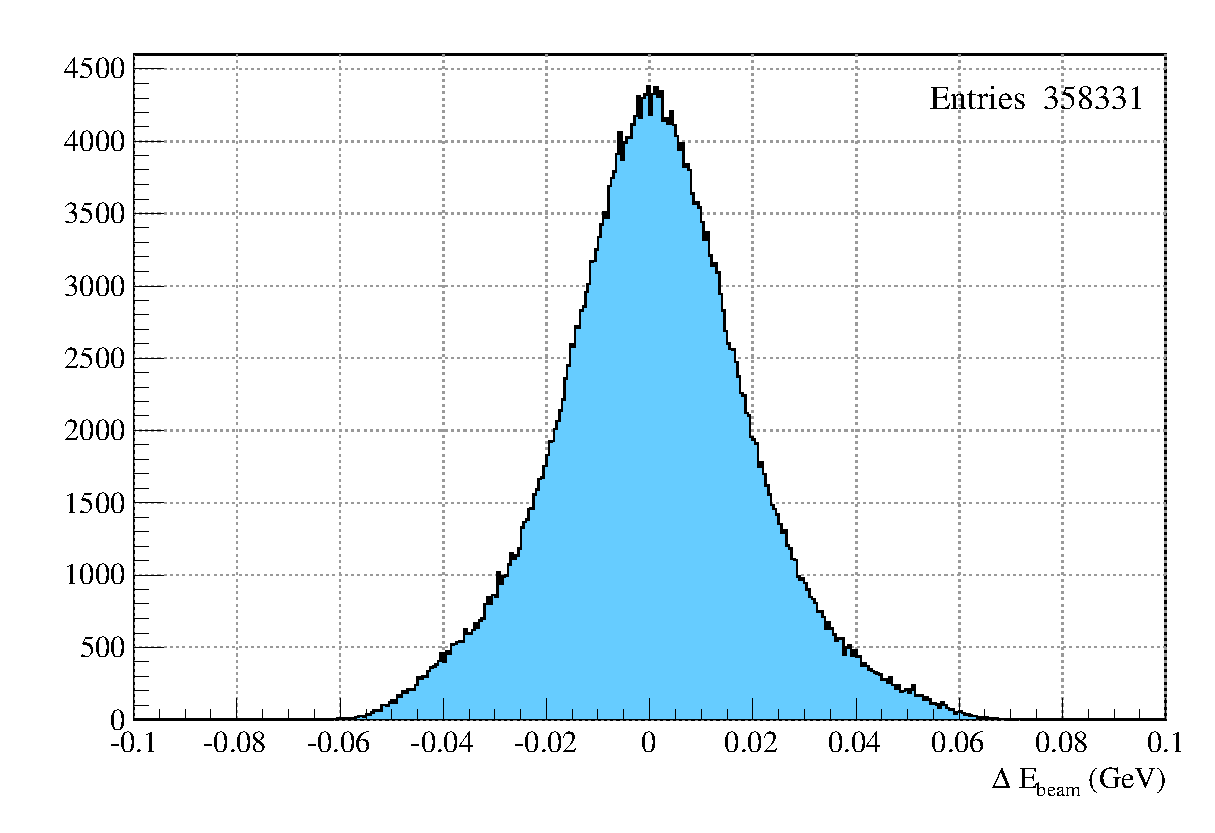
\includegraphics[width=0.7\columnwidth]{\figures/calibration/tagger/ediff_ppippim.eps}
\caption[\abbr{TAG} Energy Resolution, Overall]{\label{fig:data.calib.ediff_ppippim}The energy difference in GeV, between $E_\mathrm{beam, corrected}$ in Eq.~\ref{eqn:ebeam_ppippim}, using the exclusive reaction (\ref{rxn:excl_ppippim}) and the energy reported by the tagger. A Gaussian fit from -0.02 to 0.02~GeV gives a width of $16$~MeV.}
\end{center}\end{figure}

The resolution of the tagger time is approximately 130~ps as shown in Fig.~\ref{fig:data.calib.dttag_ppippim} and this value is used to identify the \abbr{RF} beam-bucket associated with the event. The \abbr{RF} provides the best timing resolution, on the order of a few picoseconds, in \abbr{CLAS} and it is used to calibrate the other systems as described in the sections below.

\begin{figure}\begin{center}
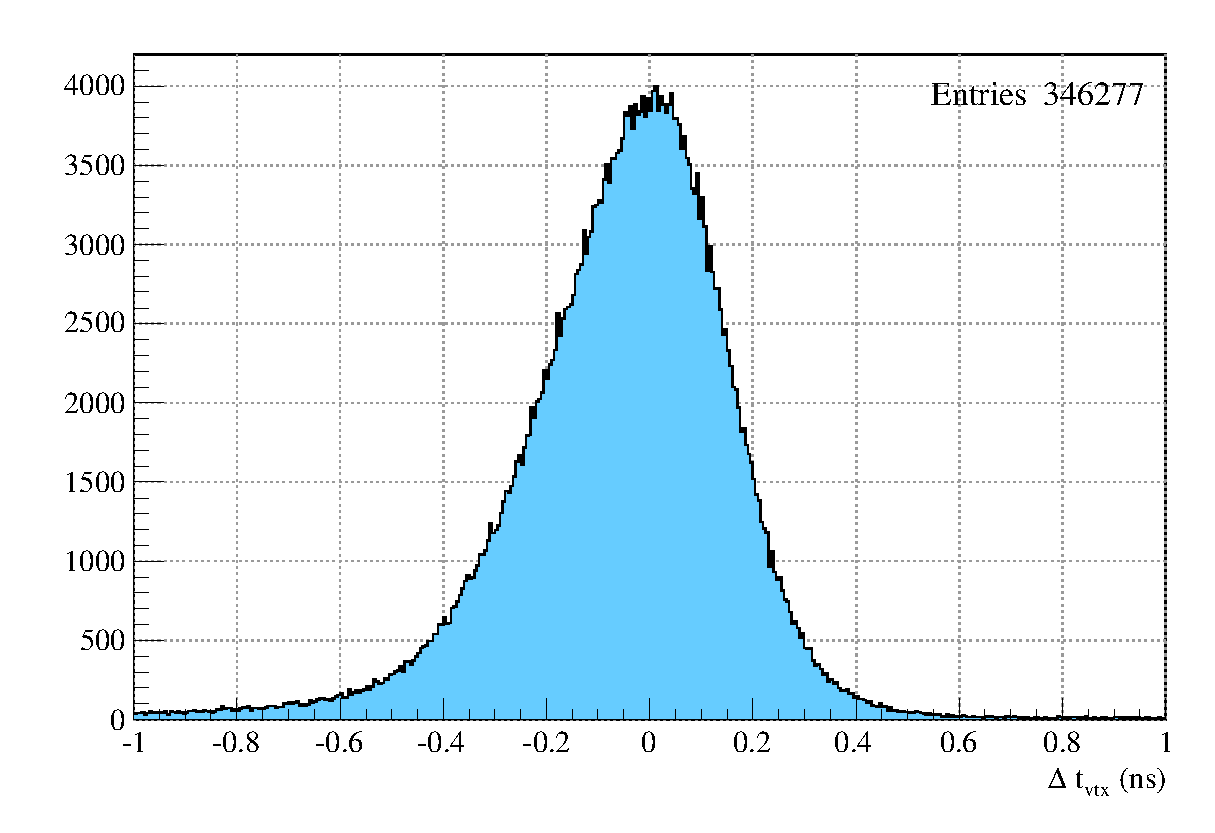
\includegraphics[width=0.7\columnwidth]{\figures/calibration/tagger/dttag_ppippim.eps}
\caption[\abbr{TAG} Timing Resolution]{\label{fig:data.calib.dttag_ppippim}The difference in time between the tagger hit and the nearest \abbr{RF} clock tick using the exclusive reaction (\ref{rxn:excl_ppippim}). A Gaussian fit from -0.2 to 0.2~ns gives a width of $130$~ps.}
\end{center}\end{figure}

The timing of the start counter (\abbr{ST}) was of critical importance for this analysis because it helped determine the tagger hit associated with the physical event. Here again, exclusive $\mathrm{p \piup^+ \piup^-}$ events were used and the tagger hit was matched to the average vertex time measured from these final state particles. The time walk ($t_\mathrm{walk}$) of the signal from the track to the \abbr{PMT} is determined by the equation:
\begin{equation}
    t_\mathrm{walk} = t_0 + \frac{t_{1}}{a - a_0},
    \label{eqn:st_timewalk}
\end{equation}
where $t_0$ and $t_1$ were determined for each paddle from the data. Here, $a$ is the \abbr{ADC} signal and $a_0$ is the \abbr{ADC} pedestal value. The difference in \abbr{ST} vertex time for the tracks and the tagger hit is shown in Fig.~\ref{fig:data.calib.st_dvtime_ppippim} and the final resolution of the \abbr{ST} was approximately 370~ps.


\begin{figure}\begin{center}
\includegraphics[width=0.7\columnwidth]{\figures/calibration/st/dvtime_ppippim.eps}
\caption[\abbr{ST} Timing Resolution]{\label{fig:data.calib.st_dvtime_ppippim}The difference in \abbr{ST} vertex time according to each of the tracks in the exclusive reaction (\ref{rxn:excl_ppippim}) and the tagger hit. A Gaussian fit from -0.5 to 0.5~ns gives a width of $370$~ps.}
\end{center}\end{figure}

The method for determining the \abbr{TOF} resolution is identical to that of the start counter. However, the time walk correction is more sophisticated owing to the finer resolution of the \abbr{TOF}:
\begin{equation}
    t_\mathrm{walk} = \left\{
      \begin{array}{ll}
            b x^{-c}
                &: a < a_1 \\
            \frac{b}{a_1^c}
                \left( b + c \left[ 1
                - \frac{\left( a - a_0 \right)}
                    {a_1 V_T}
                \right] \right)
                &: a \geq a_1
      \end{array}
      \right. ,
\end{equation}
where $t_0$, $b$ and $c$ are constants determined for each \abbr{TOF} paddle and for each calibration run range (see Table~\ref{tab:data.cook.org.runs}), $a$ is the \abbr{TOF} \abbr{ADC} signal, $a_0$ is the \abbr{ADC} pedestal value and $V_T$ is the discriminator threshold value. This equation is essentially a power law below some \abbr{ADC} value $a_1$ and a linear function above, and it has the property of being smooth at this transition point. The difference in vertex times (\abbr{TOF} and \abbr{TAG}) for the (exclusive) $\mathrm{p \piup^+ \piup^-}$ tracks is shown in Fig.~\ref{fig:data.calib.tof_dvtime_ppippim}. The \abbr{TOF} had a timing resolution of approximately 230~ps after all calibrations were completed.

\begin{figure}\begin{center}
\includegraphics[width=0.7\columnwidth]{\figures/calibration/tof/dvtime_ppippim.eps}
\caption[\abbr{TOF} Timing Resolution]{\label{fig:data.calib.tof_dvtime_ppippim}The difference in \abbr{TOF} vertex time according to each of the tracks in the exclusive reaction (\ref{rxn:excl_ppippim}) and the tagger hit. A Gaussian fit from -0.5 to 0.5~ns gives a width of $230$~ps.}
\end{center}\end{figure}

The drift-chamber was calibrated to first-order by aligning the data using the zero-field run where the particles traced a straight line. Once corrected for alignment, fixed delays and track dependent flight times were calculated to obtain the drift time of the signal from the track to each wire, given by\cite{clas.dc.calib}:
\begin{equation}
    t_\mathrm{drift} = t_\mathrm{prop} - t_\mathrm{wire}
    \label{eqn:dc_tdrift}
\end{equation}
where $t_\mathrm{prop}$ is the signal propagation time from Eq.~\ref{eqn:detector_time} and $t_\mathrm{wire}$ is the time the signal took to propagate along the wire from the point of interaction to the electronics. The drift times ($t_\mathrm{drift}$ in Eq.~\ref{eqn:dc_tdrift}) to each wire from the passing particle was then converted to a drift distance and the final tracks were determined by minimizing the absolute value of the residuals, shown in Fig.~\ref{fig:data.calib.residuals_draw}.

\begin{figure}\begin{center}
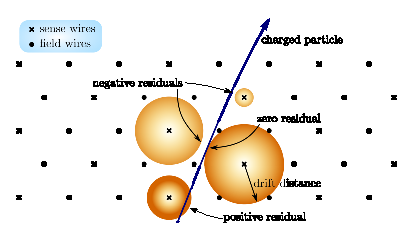
\includegraphics[width=0.85\columnwidth]{\figures/calibration/dc/residuals_drawing.eps}
\caption[\abbr{DC} Residuals Schematic]{\label{fig:data.calib.residuals_draw}Schematic of a track going through five layers of the drift chamber looking down the sense and field wires of the \abbr{DC}. Shown are the residuals obtained from the calculated drift distance, $t_\mathrm{drift}$ in Eq.~\ref{eqn:dc_tdrift}.}
\end{center}\end{figure}

The mean of the residuals is shown in Fig.~\ref{fig:data.calib.dc_res_mean}. The spread from $-50$ to 50~\um\ in the mean contributes to the overall resolution in the drift chambers. The standard deviation of the residuals in the \abbr{DC}, shown in Fig.~\ref{fig:data.calib.dc_res_sig}, was no greater than 380~\um\ for superlayer 6 --- the farthest from the target. These values combine to give a resolution of approximately 430~\um.

The maximum error of the momentum from the \abbr{DC} can be estimated by considering the constant magnetic field approximation where the particle traces a circular arc in region 2. The momentum ($p$) can be calculated from the saggita ($s$), which is described in Fig.\ref{fig:sagitta}, of the track in this region by
\begin{equation}
    p = \frac{\ell^2 q B}{8 s},
    \label{eqn:momentum_saggita}
\end{equation}
where $\ell$ is the length of the cord defined by the arc, $q$ is the charge, and $B$ is the magnetic field. The cord length was approximately 1.5~m, the charge was $\pm e$ and the magnetic field was $\sim 1$~T. If we take the resolution of the saggita ($\delta s$) to be the resolution of the residuals, then the error of the momentum ($\delta p$), which is momentum-dependent, becomes
\begin{equation}
    \delta p = \frac{8 p^2}{\ell^2 q B} \delta s.
    \label{eqn:momentum_saggita_err}
\end{equation}
This gives an approximate resolution of:
\begin{equation}
    \delta p = 0.002~\mathrm{GeV}^{-1} \times p^2.
    \label{eqn:momentum_resolution}
\end{equation}
Therefore, a 2~GeV particle going through the drift chamber should have an approximate resolution of 8~MeV. It is useful to note that this is an estimate on the \emph{maximum} error and that final momentum corrections, which are discussed in Sec.~\ref{sec:analysis.pid}, were done based on particle identification to further improve the resolution in the data.

\begin{figure}\begin{center}
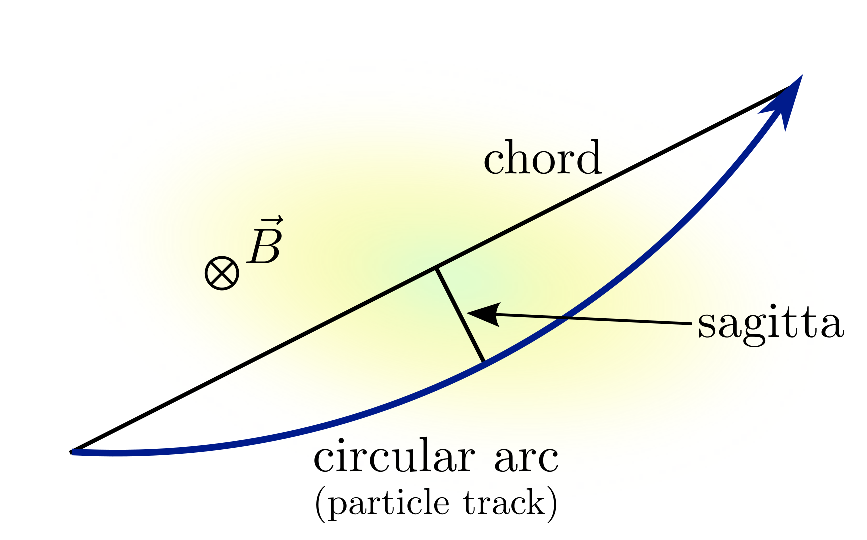
\includegraphics[width=0.45\columnwidth]{\figures/reconstruction/sagitta.eps}
\caption[Saggita of a Circular Arc]{\label{fig:sagitta}The sagitta of a circular arc is the maximum distance between the arc and a given chord. Since charged particles traveling perpendicular to a uniform magnetic field trace a circular path, this is used as an approximation for determining the maximum error of the measured momentum. Shown here is a positively charged particle moving through a uniform magnetic field ($\vec{B}$) going into the page.}
\end{center}\end{figure}

\begin{figure}\begin{center}
\includegraphics[width=0.85\columnwidth]{\figures/calibration/dc/dc_resid_mean.eps}
\caption[\abbr{DC} Resolution (Residuals, mean)]{\label{fig:data.calib.dc_res_mean}{\coloronline}Mean of residuals in the drift-chamber for each of the six superlayers. A characteristic subset of the good runs listed in Table~\ref{tab:data.cook.prodruns} were used.}
\end{center}\end{figure}

\begin{figure}\begin{center}
\includegraphics[width=0.85\columnwidth]{\figures/calibration/dc/dc_resid_sigma.eps}
\caption[\abbr{DC} Resolution (Residuals, standard dev.)]{\label{fig:data.calib.dc_res_sig}{\coloronline}Standard deviation of residuals in the drift-chamber for each of the six superlayers. A characteristic subset of the good runs listed in Table~\ref{tab:data.cook.prodruns} were used.}
\end{center}\end{figure}

\clearpage
